\documentclass{article} % For LaTeX2e
\usepackage{iclr2027_conference,times}

% Optional math commands from https://github.com/goodfeli/dlbook_notation.
\input{math_commands.tex}

\usepackage{hyperref}
\usepackage{url}
\usepackage{enumitem}
\usepackage{amsmath}
\usepackage{mathtools}
\usepackage[table]{xcolor}
\usepackage{pgf}
\usepackage{collcell}
\usepackage{multirow}
\usepackage{cleveref}

\DeclarePairedDelimiter{\set}{\{}{\}}

% Passes colorblind
\definecolor{heatLo}{HTML}{c7101b}  % dark, red
\definecolor{heatMid}{HTML}{F5F0E1}
\definecolor{heatHi}{HTML}{6BE59A}  % light green

\newcommand{\heatTint}{60}          % % of colour kept; rest is white

% \heatbg{lo}{hi}{value}: sets the cell colour only
\newcommand{\heatbg}[3]{%
  \pgfmathsetmacro{\heatT}{max(0,min(1,((0#3)-(#1))/((#2)-(#1))))}%
  \ifdim\heatT pt<0.5pt
    \pgfmathsetmacro{\heatP}{200*\heatT}\edef\heatCol{heatMid!\heatP!heatLo}%
  \else
    \pgfmathsetmacro{\heatP}{200*\heatT-100}\edef\heatCol{heatHi!\heatP!heatMid}%
  \fi
  \edef\heatDo{\noexpand\cellcolor{\heatCol!\heatTint!white}}\heatDo}
\newcommand{\heatcell}[3]{\heatbg{#1}{#2}{#3}#3}
\newcommand{\heatcellmath}[3]{\heatbg{#1}{#2}{#3}$#3$}

% Generic types: H{lo}{hi} prints as text, M{lo}{hi} prints in math mode
\newcolumntype{H}[2]{>{\collectcell{\heatcell{#1}{#2}}}r<{\endcollectcell}}
\newcolumntype{M}[2]{>{\collectcell{\heatcellmath{#1}{#2}}}r<{\endcollectcell}}

% Paper presets
\newcolumntype{P}{H{0.0}{1.0}}  % Probe Skill
\newcolumntype{E}{M{-1.0}{1.0}} % Edit Index (signed)
% \newcolumntype{F}{H{2.5}{0.0}}  % Fidelity Ratio

\newcommand{\heatcellinv}[3]{%
  \pgfmathsetmacro{\heatVal}{1-(#3)}%
  \heatbg{#1}{#2}{\heatVal}%
  \pgfmathprintnumber[fixed,precision=2,showpos]{\heatVal}%
}

\newcolumntype{I}[2]{>{\collectcell{\heatcellinv{#1}{#2}}}r<{\endcollectcell}}

% Example preset
\newcolumntype{F}{I{-1.0}{1.0}}

\newcolumntype{G}{@{}p{10pt}@{}}


\title{When Generative Models Act as Simulators}

% Authors must not appear in the submitted version. They should be hidden
% as long as the \iclrfinalcopy macro remains commented out below.
% Non-anonymous submissions will be rejected without review.

\author{
}

% The \author macro works with any number of authors. There are two commands
% used to separate the names and addresses of multiple authors: \And and \AND.
%
% Using \And between authors leaves it to \LaTeX{} to determine where to break
% the lines. Using \AND forces a linebreak at that point. So, if \LaTeX{}
% puts 3 of 4 authors names on the first line, and the last on the second
% line, try using \AND instead of \And before the third author name.

\newcommand{\fix}{\marginpar{FIX}}
\newcommand{\new}{\marginpar{NEW}}
\newcommand{\red}[1]{\textcolor{red}{#1}}

% \iclrfinalcopy % Uncomment for camera-ready version, but NOT for submission.
\begin{document}


\maketitle

\begin{abstract}
% Begin with a definition of simulators
% Carrying out waht if experiments -- I would like my model as such that if my representation of the world through the state is such that if I can play what if scenatios then I can 
% Acknowledge that the state of the world is not an intrinsic thing -- discuss 
Generative models can learn to produce novel observations from an environment by training on sampled output sequences. 
% Drop "frmo an environment"
% In the case where the observations come from a dynamical process we call a simulator a process which can produce the next step
% A simulator has a state which a simpler (interpretable) condensed of the bservations and we care about the ability to set this state
Many use cases for such models, \textit{e.g.} agentic training, planning, or counterfactuals, depend on viewing them as environment simulators.
For a generative model to act as a simulator, we require an ability to set its latent representation so that its predictions match the environment’s outputs from a target environment state. We call this capability \textit{editability}, and focus here on next-step predictions.
Holding the architecture, training setup, and evaluation fixed, we show that small environmental changes meaningfully affect a generative model’s editability, and thus whether it can be used as a simulator.
% We begin with the approach of training probes to decode environment state from the learned latent space, then test whether these probes can guide targeted edits.
We train linear and MLP probes to decode environment state from the learned latent space, then test whether their associated editors can make targeted changes to the model’s output.
Our tested environments fall into two broad classes: the game of Othello and an environment with moving discs rendered into partial 1D observations, which we call Rayworld. In Othello, we demonstrate that changing specific game rules can toggle the editability of a learned model. In our Rayworld experiments, decoding probes find increasingly steerable representations when observation resolution is decreased and the state is represented categorically, as in Othello, rather than as continuous positions. We further train an MLP to learn a direct mapping from the environment state to the latent state and find that it can drive the output when decoding probes cannot, even when it predicts latent states poorly.
Our results show that probe-derived editing is not sufficient to make claims about whether a generative model can act as a simulator.
\end{abstract}


% #####################################################################
\section{Introduction}

\begin{figure}[b]
\centering
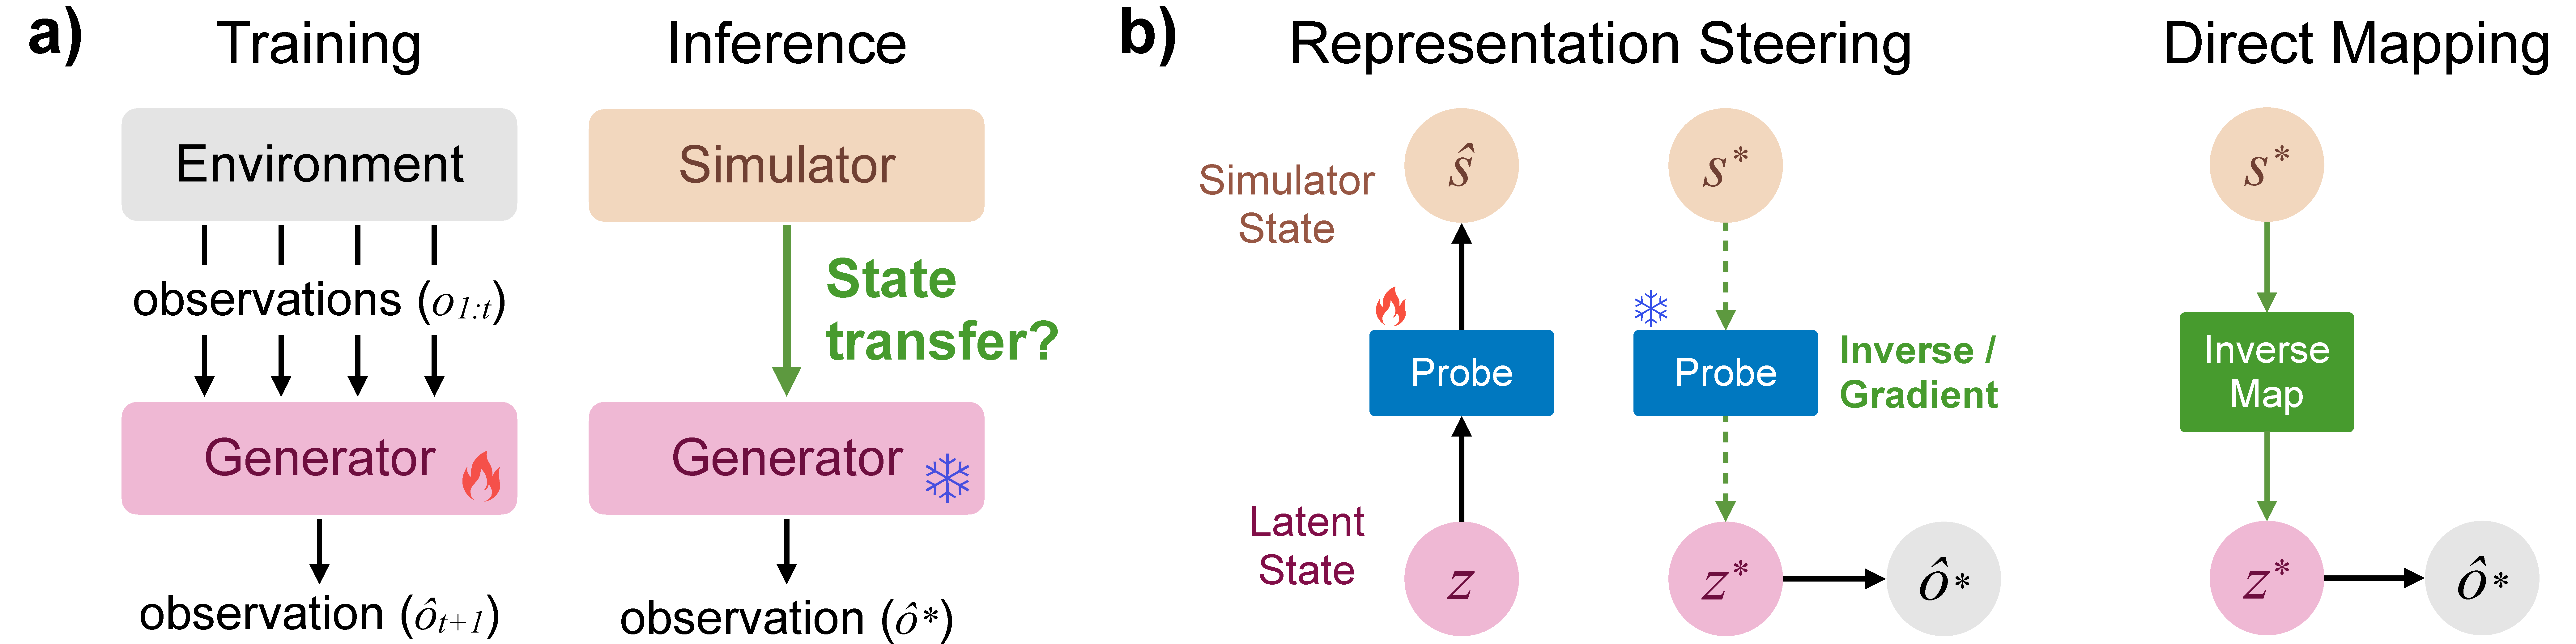
\includegraphics[width=0.95\linewidth]{figs/teaser.pdf}
\caption{Overview of the paper's main points.Overview of the paper's main points.Overview of the paper's main points.Overview of the paper's main points.Overview of the paper's main points.}
\label{fig:teaser}
\end{figure}

A simulator represents an environment by holding a state, advancing it by a rule, and rendering it into observations. In conventional simulators, this state is explicit and interpretable, allowing it to be set while preserving commitments to that environment and its rules \citep{blank_cite}. What these systems can express, however, is constrained by what has been specified. Generative models, by contrast, learn from observations and can supply plausible details where that specification is incomplete \citep{blank_cite}. If an observer has seen only half of a room and then turns around, a generative model can propose what lies behind them, consistent with what they have already seen \citep{blank_cite}. Their internal representations, however, typically offer no straightforward means of setting that environment’s state \citep{blank_cite}.

One step toward combining the strengths of generators and simulators is to understand when a generator’s learned representations support the same kind of state-setting interface as a simulator. We study the model’s \textit{editability} with respect to particular environment variables by testing whether direct interventions to its latent state produce the output changes expected from an edit to those variables. This is a question about the functionality we can access, without requiring that the model internally represents or advances state in the same way as a conventional simulator. Our experiments examine the effect of an edit on next-step predictions.

The conditions under which an environment variable becomes editable are not apparent from decodability alone. A variable may be accurately decoded from a model’s representations without the decoding probe providing a means of changing its effect on the output \citep{blank_cite}. We investigate this distinction by holding the model architecture, training setup, and evaluation fixed while varying properties of the training environment. Changing the rules governing a variable, or the observations through which it is revealed, allows us to test which conditions support control over that variable. Such comparisons can help distinguish limitations of the model’s learned capabilities from limitations of the procedures used to access them.

We study two classes of environment: the game of Othello, where observations are move sequences and state is a discrete board configuration \citep{blank_cite}, and Rayworld, where moving discs are rendered into partial 1D observations. We vary the game rules in Othello and the observation process in Rayworld, and also compare continuous and categorical descriptions of the discs’ state. To make comparisons across these settings, we introduce a unified evaluation of decodability and editability using access to ground truth simulators implementing each environment. Our metrics quantify state recovery relative to a trivial predictor and measure whether an intervention moves the output toward that of the edited environment state while preserving quality.

For each environment, we train linear and MLP probes to decode its state from the trained model’s latent representations. Each probe is paired with an editor that uses it to guide changes to those representations. When these edits succeed, the probe has provided an effective handle for controlling the model’s output. When they fail, however, the model may still support the desired state change through another means. To investigate this gap, we train an inverse mapping directly from environment state to latent representation and use its prediction to overwrite the model’s latent state. This tests whether the model can act as a simulator even when the representations identified by decoding probes do not provide effective editing handles.

Across our environment variants, strong decodability coexists with substantial differences in editability. In Othello, changing the game rules can prevent all three tested editors from controlling a variable, even when that variable remains relevant to predicting legal moves. In Rayworld, probe-derived editing of continuous positions remains weak, but becomes increasingly effective when the state is described categorically and observations are made coarser. The inverse mapping succeeds across all the tested Rayworld variants, including cases where it predicts latent states poorly ($R^2=0.34$), while accurate latent prediction in some Othello variants does not yield successful edits. Thus, faithfully reconstructing the model’s latent state is neither necessary nor sufficient for the inverse mapping to provide effective control.
%By varying the environment, we investigate when learned variables become accessible to intervention, distinguishing control exposed by decoding probes from the broader capacity to act as a simulator.

Our main contributions are as follows:
\begin{enumerate}[
label=(\arabic*),
leftmargin=*,
align=left,
itemsep=0.25em,
topsep=0pt,
parsep=0pt,
partopsep=0pt
]
\item \textbf{A unified methodology for evaluating decodability and editability across environments}
\item \textbf{A controlled study of when probes find steerable representations as environments vary}
\item \textbf{A demonstration that inverse mappings can steer models when probe-derived editors fail, even when they predict latent states poorly}
\end{enumerate}


% #####################################################################
\section{Background}

\subsection{World Models and Simulators}

World models provide learned environments for agent training \citep{ha2018worldmodels}. Video generators are increasingly presented as a route to world simulation, including Sora, Genie, and Cosmos \citep{brooks2024sora,bruce2024genie,nvidia2025cosmos}. However, accurate generation alone does not establish that internal representations correspond to environment states and support their manipulation.

Identifiability theory concerns whether observed distributions determine latent structure up to specified transformations. Unsupervised disentanglement requires inductive assumptions \citep{locatello2019disentanglement}, while auxiliary observations can enable identification under suitable conditions \citep{khemakhem2020identifiability}. We study the readout and editability of particular trained representations, rather than uniqueness of the latent explanation.

\citet{vafa2024evaluating} test whether sequence continuations preserve equivalences and distinctions between environment states, while \citet{kang2025physical} evaluate generalization of physical laws through generated trajectories. Recent studies also decode physical variables from video encoders and generators, with interventions evaluated through probe readouts or probe-assessed plausibility \citep{joseph2026physics,esmati2026invisible}. % Needs a note on what makes ours different.

Control over generation can be supplied through trained conditioning interfaces \citep{zhang2023controlnet,li2023gligen,wang2024motionctrl,he2024cameractrl,nvidia2025transfer} or an explicit physical simulator \citep{zhang2024physdreamer}. We instead evaluate whether representations learned through next-step prediction support state edits whose outputs match the corresponding simulator intervention, without training the generator to accept state controls.

\subsection{Probing and Steering Learned Representations}

Othello provides a concrete demonstration of editable environment representations. Players place discs and flip enclosed opponent discs on a board, as detailed in \cref{sec:othello_experiments}. \citet{li2023othello} decode board states from a transformer trained on move sequences and use probe gradients to change its move predictions toward those of edited boards. \citet{nanda2023linear} show that representing disc ownership as mine/theirs makes the board linearly decodable and enables edits through vector arithmetic.

Decodability does not establish how a model uses the decoded information. Probe controls distinguish information recovery from the probe's own learning \citep{hewitt2019probes}, and amnesic probing measures behavioral changes after removing linearly accessible information \citep{elazar2021amnesic}. Intervention reliability also depends on changing the target while preserving other properties \citep{canby2025reliable}. Decoder weights need not follow the activation patterns that encode a variable, motivating covariance-based corrections \citep{haufe2014interpretation}. Activation steering has a prominent LLM literature \citep{zou2023repe,rimsky2024caa}, alongside earlier semantic editing of image generators \citep{shen2020interfacegan}. We hold probe and editor families fixed across controlled environment variants to study how the environment affects both readout and simulator-grounded editing.

\subsection{Causal Abstraction}

Causal abstraction formalizes correspondence between systems through matched interventions \citep{geiger2021causal,geiger2025foundation}. Interchange interventions replace aligned internal components with values from another execution, and interchange intervention accuracy measures agreement with the corresponding high-level outcome. Distributed Alignment Search learns a rotation that exposes aligned subspaces by optimizing intervention outcomes while keeping the analyzed model fixed \citep{geiger2024das}. Our evaluation follows this intervention-based view of correspondence. Our editors are fitted from state--activation pairs, rather than optimized against counterfactual output targets, and our metrics measure output distances rather than exact agreement. We study the performance of these fixed editing procedures across environments, without claiming that their failure rules out a causal abstraction under another alignment.

\subsection{Observability and Control Theory}

Observability concerns recovering state from output histories and known inputs, while controllability concerns reaching states through admissible inputs \citep{astrom2008feedback}. Our decodability instead measures recovery of environment state from a learned activation using a specified probe class. Our editability evaluates direct activation interventions against simulator counterfactuals, rather than reachability through the system's dynamics. These terms describe empirical properties of a model and analysis procedure, not classical observability or controllability guarantees.

% #####################################################################
\section{Experimental Setup}

Our experiments hold model training and analysis fixed while varying properties of the environment. Every model is a transformer of the same size, trained with the same recipe on the same number of sequences to predict the next observation, and every model is read with the same probes, written to with the same editors, and scored with the same metrics. A difference between rows of our tables is therefore a fact about the environment the training data came from. Our environmental variations are applied within two categories: the game of Othello, and a 2D world of simple objects which we refer to as Rayworld. The two are varied along different axes on purpose. In Othello the state is fully determined by the input, so the only thing worth varying is what the dynamics do with it. In Rayworld the dynamics are linear and fixed, so the only thing worth varying is what the observation reveals. Each environment varies the axis it has.

\subsection{Othello}
\label{sec:othello_experiments}

\begin{figure}[t]
\centering
\fbox{\parbox{0.9\linewidth}{\centering \vspace{15em} \red{Placeholder: visualization of the different environment variants for Othello.} \vspace{3em}}}
\caption{In standard Othello (a), two players alternate placing tiles which must bookend tokens of their opponents tiles, causing them to flip color, and the model is trained to predict the distribution over next legal moves. We experiment with changing the placement rule to require only being adjacent to a token of your own color with flipping kept on (b), or with flipping turned off (c), and finally with the original placement rules but no flipping, which results in a fixed checkerboard pattern being played but in different sequence across games (d). Details in \cref{sec:othello_experiments}.}
\label{fig:othello_and_variants}
\end{figure}

In the game of Othello players alternate placing discs on an $8 \times 8$ board, where a legal move must enclose opponent discs along a line (including diagonal), and the enclosed discs flip color. We follow \citet{othellogpt}, who trained a transformer on synthetic Othello games and edited the board decoded from its residual stream, and \citet{nanda}, who showed the board is linearly decodable when represented in terms of mine/theirs, with respect to the active player, instead of black/white. Our games come from the same generator of \citet{othellogpt}, which draws every move uniformly from the legal set $L_t$, so the cross entropy has an exact floor of $\mathbb{E}[\log |L_t|]$ and the optimal model must learn a uniform distribution over all legal moves.

The state in all Othello variants is the 64-grid board after each move, with each cell being classified as empty, the mover's (mine), or the opponent's (theirs). The edit target is to flip the color of a single token after opening with a real game sequence, scored against the true legal sets before and after the flip. A visualization of the Othello setup can be found in \cref{fig:othello_and_variants}

\subsubsection{Othello Variants}
We introduce three variants to the typical Othello environment. In \texttt{adjacent-flip} we keep the standard flipping rule, but modify the placement rule such that tokens must only be directly adjacent to an existing token of the same color (including diagonally). Therefore, flips appear and affect the legal move distribution, but are rarer and incidental (0.27 flipped tokens per move, against 2.2 in standard Othello). Our second variant, \texttt{adjacent-noflip}, keeps the same placement rule as adjacent-flip, but also turns off flips so that placed tokens never have their color changed over the course of a game. Finally, we test a variant called \texttt{standard-noflip} which uses the original placement rules of enclosing lines of opposite tokens, but turns off the flipping process. Note that under this setup the games are always played out as an identical checkerboard pattern, although the order of moves still has substantial variation. Color is then fixed by the square a token sits on, so it is entangled with the board geometry rather than being a variable in its own right. A visualization of our Othello variants can be found in \cref{fig:othello_and_variants}.

\subsection{Rayworld}
\label{sec:rayworld_experiments}

\begin{figure}[t]
\centering
\fbox{\parbox{0.9\linewidth}{\centering \vspace{15em} \red{Placeholder: visualization of the different environment variants for Rayworld.} \vspace{3em}}}
\caption{In standard Rayworld (a) two discs are initialized with random positions and velocities, and then move within a 2D frustum, never colliding with each other or the walls. The discs are rendered into a 1D observation at each timestep by casting rays into the frustum, and the model is trained to predict next-step observations given the preceding sequence. We experiment with adding signaled blinking periods where discs turn invisible for several turns (b), coarsening the observation process by reducing the number of rays (c), and changing the state representation from continuous positions to discrete categories (e). Details in \cref{sec:rayworld_experiments}.}
\label{fig:rayworld_and_variants}
\end{figure}

In our Rayworld environments, an observer at the origin looks into a 2-dimensional trapezoidal frustum in which two discs move at constant velocity for 40 frames, with trajectories where the discs collide with the walls or each other rejected, so the dynamics are exactly linear. A 1-dimensional observation is formed by a nonlinear rendering process on each frame without noise. To render, we cast 128 rays uniformly in the tangent of the viewing angle, each returning the reflectivity of the nearest disc it hits ($0.4$ or $0.8$, fixed per disc) or $0$ if it misses both discs, with one pixel per ray. Depth is never observed directly and enters only through the number of rays a disc covers, due to the geometric spreading of rays, and through occlusion. A visualization of the Rayworld setup is shown in \cref{fig:rayworld_and_variants}

The state in Rayworld is composed of the 2D position and velocity of both discs, and predicting the next frame decomposes as a belief over it,
\begin{gather}
\mathbf{x}_t = \begin{bmatrix} p_{1,t} & v_{1,t} & p_{2,t} & v_{2,t} \end{bmatrix}^\top \in \mathbb{R}^8, \qquad
\mathbf{x}_{t+1} = A\,\mathbf{x}_t, \qquad \mathbf{y}_t = h(\mathbf{x}_t) \in [0,1]^R, \\
\hat{\mathbf{y}}_{t+1} = \mathbb{E}[\mathbf{y}_{t+1} \mid \mathbf{y}_{1:t}] = \int h(A\,\mathbf{x}_t)\, p(\mathbf{x}_t \mid \mathbf{y}_{1:t})\, d\mathbf{x}_t,
\end{gather}
where $A$ advances each position by its velocity and $h$ is the nonlinear rendering function. Nothing in this identity forces a predictor to represent the state, and whether it does is what the probes and editors investigate. We probe the state in the Cartesian coordinates the dynamics act in, so the probe target is the quantity $A$ advances.

The edit target for all Rayworld variants is a teleportation of one disc at frame 20 of a held-out sequence to a random position clear of the walls and the other disc. The velocities of both objects are held constant. We warm the model on frames 0 to 19, edit its residual stream at the last frame, and score its prediction of the edited frame 20.

\subsubsection{Rayworld Variants}
We introduce four variants of the Rayworld environment. The first variant, \texttt{smooth}, changes how a disc is drawn onto the rays it covers. Instead of every covered ray reading the disc's full reflectivity, the value falls off from the disc's center to its edge (a continuous half-dome, details in \cref{app:rw_smooth_dome}), so the values on the covered rays shift continuously with the disc's sub-pixel position. Depth still only enters in the apparent width of the disc, but the observation now determines position more precisely. Our second variant, \texttt{obs5}, increases the number of observers from one to five, each with the 8-ray observation described below, so the observation is five views side by side. The observers are equally spaced in a ring around the arena, and the discs are constrained to always lie within the circle carved by the near and far ranges of each observer. Our next variant, \texttt{blink}, introduces random `blinking' periods where a disc turns invisible for 1 to 12 frames, with the start and end of a blink signaled to the model. Finally, our last variant is actually a class of variants which we refer to as \texttt{N-ray}. In each of these variants we quantize the observations by reducing the number of rays cast, which also reduces the dimensionality of the observations. We test this variant for $N \in \set{5, 8, 16}$, and double the disc radius so that a disc always covers at least one ray. A visualization of our Rayworld variants can be found in \cref{fig:rayworld_and_variants}.

\subsection{Model, training, and probes}

Every model trains on 20M sequences (with 10\% used for validation) for 780,000 steps at batch size 256 from one seed. The probes used are a linear map and an MLP with one hidden layer of dimension 128, fitted at every residual point on roughly 1.2M pairs of latent state and environment state, and held out by sequence. Continuous targets are fit by minimizing squared error, in closed form for the linear probe and by gradient descent for the MLP. Categorical targets are fit by minimizing cross entropy. The probe targets are the mine/theirs board in Othello and the eight-dimensional state in Rayworld, with probe inputs standardized.

We also test a categorical version of the Rayworld target, so that Rayworld can be probed and edited the same way as Othello. In Rayworld, each disc lights up a short run of adjacent rays. The center of the run depends on the disc's lateral position and its length depends on the disc's depth. Only a finite number of different runs are possible, so we treat each run as a cell and label every cell as empty, containing disc one, or containing disc two. We call this the appearance target, since two positions fall in the same cell exactly when the disc looks the same. Under this target an edit moves a disc from one cell to another, just as an Othello edit changes one square. We report a factorized version of this target. Instead of one label per cell, the probe predicts for each disc separately one categorical variable for the center of its run and one for its length (15 and 5 classes on the 8-ray variant). The partition is the same, but an edit now changes the two labels of the moved disc rather than emptying one cell and filling another, and the number of outputs stays small even when the partition is fine. The categorical probes are fit on a larger corpus of 200,000 sequences, to account for the increase in parameters.

\subsection{Editors}

An editor changes the residual stream at the most recent position, and the model then predicts from the changed stream. With $\mathbf{z}$ the standardized latent state at one residual point, $f_{\mathrm{Lin}}(\mathbf{h}) = W\mathbf{z} + \mathbf{b}$ the linear probe, $f_{\mathrm{MLP}}(\mathbf{h})$ the MLP probe, and $\mathbf{s}$ the target environment state,
\begin{align}
\text{PI:}\quad & \Delta\mathbf{h} = W^{+}(\mathbf{s} - f_{\mathrm{Lin}}(\mathbf{h})), \qquad \mathbf{h}' = \mathbf{h} + \alpha\,\Delta\mathbf{h}, \\
\text{GS:}\quad & \mathbf{h} \leftarrow \mathbf{h} - \eta\, \nabla_{\mathbf{h}}\, \mathcal{L}\big(f_{\mathrm{MLP}}(\mathbf{h}), \mathbf{s}\big), \\
\text{IM:}\quad & \mathbf{h}' = g(\mathbf{s}).
\end{align}
Pseudoinverse injection (PI) makes the smallest change to the latent state, measured in standardized units, that moves the linear probe's reading onto the target, and $\alpha$ scales that change, with $\alpha = 1$ landing exactly. PI writes at one residual point and every later layer runs unchanged. Gradient steering (GS) takes 100 gradient steps on the latent state so that the MLP probe's reading approaches the target, with the probe's own loss as $\mathcal{L}$, which also penalizes changes to the unedited entries at a lower weight. GS writes at a starting layer and again at every later residual point. Inverse mapping (IM) runs the probe in reverse. We fit a map $g$ from environment state to latent state, an MLP with the same size and training recipe as the forward probe, and at edit time replace the latent state entirely with $g(\mathbf{s})$. IM writes at one residual point and has no step size. To check that $g$ learns an inverse process rather than memorizing training states, we compare it against overwriting with the mean latent state of the nearest training states, which IM beats by \red{XX.X\%} on average (\cref{app:inverse_nearest_neighbor}). For each editor we sweep the residual point (and step size where there is one) and report the outcome with the highest Edit Index alongside its Fidelity Ratio. Every model is scored on a bench of 1000 edit cases built the same way for its instance. Each case is a held-out sequence cut at step 20, a 20-move prefix in Othello or frame 20 in Rayworld, with one variable changed, and cases whose edit leaves the observation unchanged (an identical legal set, or fewer than two rays) are skipped.

\subsection{Metrics}

We introduce a common metric called Probe Skill to measure decodability. The formula we use is $1.0$ minus the probe loss divided by the loss of a trivial predictor. For continuous targets we use MSE loss and a constant mean for the trivial predictor, which becomes exactly the $R^2$ formula. For discrete categorization we use mean misclassification rate as the loss, and use a per-variable majority class rule as the trivial predictor. For every probe and trained model we also compare against two baselines: the same probe trained on a randomly initialized model, and trained directly on the raw observation sequences.

We introduce a second metric called the Edit Index to measure editability. The idea is to compare the model's output after a latent edit against two reference outputs, one for the world where the edit happened and one for the world where it did not, and ask which the output is closer to. Both references come from the simulator. In Rayworld they are the rendered frames of the edited and unedited worlds at the edit step. In Othello they are the uniform distributions over the legal moves of the board before and after the flip, which is the exact optimal prediction since the game generator is uniform. We compute the RMSE from the model's output $\hat{o}$ to each reference, restricted to the rays whose rendered value differs between the two worlds, or the squares whose legality the flip changes, and call these $d_{\mathrm{edit}}$ and $d_{\mathrm{uned}}$. Because the index only measures relative distance, we pair it with the Fidelity Ratio, which compares the edited output's error to the error the model had with no edit at all. The formulae are then
\begin{align}
\text{Edit Index} = \frac{d_{\mathrm{uned}} - d_{\mathrm{edit}}}{d_{\mathrm{uned}} + d_{\mathrm{edit}}}, \qquad
\text{Fidelity Ratio} = 1- \frac{\operatorname{RMSE}(\hat{o}^{\mathrm{edited}}, o^{\mathrm{edit}})}{\operatorname{RMSE}(\hat{o}^{\mathrm{unedited}}, o^{\mathrm{edit}})}.
\end{align}
An Edit Index of $+1$ means the output matches the edited world, $-1$ means it matches the unedited world, and a value near $0$ means it is equally far from both. This last case includes a destroyed output, so the index alone cannot distinguish promising-but-small edits from destructive ones, which is what the Fidelity Ratio determines. A Fidelity Ratio above $1.0$ means the edit made the prediction worse than doing nothing, and we do not count such an edit as a success. As a sanity check on the index itself, we score the model on a history that genuinely produces the edited world, by re-rendering the entire input sequence with the disc teleported in Rayworld, and by finding a real game whose board equals the flipped board in Othello. Both reach \red{$+0.91$}. The remaining gap represents the model's inherent prediction error, which is why these metrics are meant for models that already predict well, as we verify in \cref{app:predict_skill}.


% #####################################################################
\section{Results}

We report decodability for every run in \cref{tab:decodability}, editability in \cref{tab:editability}, and editability through the categorical Rayworld target in \cref{tab:appearance_fac}. Every model is a strong predictor of its environment before any probing or editing begins, with the Othello models within \red{$0.02$} nats of their exact floors and the Rayworld models at held-out squared errors below \red{$0.006$} (full scores in \cref{app:predict_skill}).

\newcommand{\lightrule}{%
  \noalign{\global\arrayrulewidth=0.25pt}%
  \arrayrulecolor{black!35}\hline
  \arrayrulecolor{black}%
  \noalign{\global\arrayrulewidth=0.4pt}}

\begin{table}[t]
\centering
\small
\setlength{\tabcolsep}{4pt}
\begin{tabular}{ll PP G PP G PP G PP}
\hline
\noalign{\vspace{0.25em}}
& & \multicolumn{11}{c}{Probe Type} \\
\noalign{\vspace{0.25em}}
\cline{3-13}
\noalign{\vspace{0.25em}}
& & \multicolumn{2}{c}{Observation} & & \multicolumn{2}{c}{Random init} & & \multicolumn{2}{c}{Trained} & & \multicolumn{2}{c}{Inverse Map MLP} \\
Class & Variant
& \multicolumn{1}{c}{Lin.} & \multicolumn{1}{c}{MLP} & &
\multicolumn{1}{c}{Lin.} & \multicolumn{1}{c}{MLP} & &
\multicolumn{1}{c}{Lin.} & \multicolumn{1}{c}{MLP} & &
\multicolumn{1}{c}{Best Point} & \multicolumn{1}{c}{Edit Point} \\
\hline
\noalign{\vspace{0.1em}}
\multirow{4}{*}{Othello}
& standard        & 0.792 & 0.809 & & 0.577 & 0.583 & & 0.975 & 0.976 & & 0.884 & 0.827 \\
& adjacent-flip   & 0.888 & 0.914 & & 0.674 & 0.700 & & 0.947 & 0.970 & & 0.968 & 0.959 \\
& adjacent-noflip & 0.988 & 0.983 & & 0.581 & 0.588 & & 0.988 & 0.990 & & 0.978 & 0.970 \\
& standard-noflip & 1.000 & 1.000 & & 1.000 & 1.000 & & 1.000 & 1.000 & & 0.947 & 0.944 \\
\cline{1-13}
\multirow{5}{*}{Rayworld}
& standard & 0.305 & 0.885 & & 0.738 & 0.945 & & 0.872 & 0.973 & & 0.741 & 0.339 \\
& blink    & 0.216 & 0.809 & & 0.608 & 0.870 & & 0.907 & 0.979 & & 0.613 & 0.338 \\
& 16-ray   & 0.360 & 0.907 & & 0.890 & 0.949 & & 0.892 & 0.965 & & 0.554 & 0.516 \\
& 8-ray    & 0.329 & 0.877 & & 0.883 & 0.919 & & 0.886 & 0.932 & & 0.585 & 0.580 \\
& 5-ray    & 0.277 & 0.829 & & 0.855 & 0.871 & & 0.850 & 0.883 & & 0.617 & 0.469 \\
\hline
\end{tabular}
\caption{Decodability (higher is better), measured as Probe Skill for each environment variant. We report scores at the trained model’s best residual point, alongside random-initialization and observation-space baselines fitted with the same probes on the same sequences. The Inverse Map MLP predicts latent state from environment state. For this mapping, Best Point reports its highest prediction score across residual points, while Edit Point reports its prediction score at the residual point where it achieves the highest Edit Index. Details in \cref{sec:decoding_results}.}
\label{tab:decodability}
\end{table}


\subsection{Decodability}
\label{sec:decoding_results}

The environment state is decodable in every instance we test. The MLP probe reaches a Probe Skill of at least $0.88$ on every model, and the linear probe is close behind. What separates the instances are the baselines. In Othello, the trained model beats both baselines by a wide margin only when flipping is on, at $0.975$ against $0.58$ and $0.79$ for the standard game and $0.947$ against $0.67$ and $0.89$ for \texttt{adjacent-flip}. Without flipping the board can be read directly from the move sequence, so the \texttt{adjacent-noflip} model matches its observation baseline at $0.988$ and every probe on \texttt{standard-noflip} scores a perfect $1.000$, including the one fitted to a randomly initialized model. In Rayworld the random initialization baseline sits within $0.05$ of the trained model for every variant except \texttt{blink}, where it falls to $0.87$ against $0.98$. % Discuss generally low observation decodability for rayworld
Its observation baseline is among the lowest as well, since a disc that is currently invisible cannot be located from the observations alone, \red{so \texttt{blink} is the one Rayworld variant where the model must carry position in its latent state rather than reading it off the current frame.} % Too strong of a statement

\subsection{Editability}
\label{sec:editing_results}

Standard Othello is editable by every editor, replicating \cref{othellogpt}. PI, GS, and IM all reach an Edit Index between $+0.81$ and $+0.83$ against an unedited score of $-0.93$, with Fidelity Ratios of $0.28$ to $0.38$, so each edit moves the predicted move distribution most of the way to the flipped board. Every variant of the rules changes this. With flipping turned off, no editor lands on either no-flip variant. The best indices come only from writes that destroy the prediction, with Fidelity Ratios of $1.48$ and above, and this holds for \texttt{adjacent-noflip} even though its legal moves depend on token color. Restoring flips under the adjacency rule restores editability for IM alone, at $+0.66$ with a Fidelity Ratio of $0.51$, while PI and GS reach modest index scores only at ratios above $1.7$.

\begin{table}[t]
\centering
\small
\setlength{\tabcolsep}{4pt}
\begin{tabular}{ll E G EF G EF G EF}
\hline
\noalign{\vspace{0.25em}}
& & \multicolumn{1}{c}{} & & \multicolumn{8}{c}{Edit Type} \\
\noalign{\vspace{0.25em}}
\cline{5-12}
\noalign{\vspace{0.25em}}
& & \multicolumn{1}{c}{Unedited} & & \multicolumn{2}{c}{PI} & & \multicolumn{2}{c}{GS} & & \multicolumn{2}{c}{IM} \\
Class & Variant & \multicolumn{1}{c}{Index} & &
\multicolumn{1}{c}{Index} & \multicolumn{1}{c}{Fid.} & &
\multicolumn{1}{c}{Index} & \multicolumn{1}{c}{Fid.} & &
\multicolumn{1}{c}{Index} & \multicolumn{1}{c}{Fid.} \\
\hline
\noalign{\vspace{0.1em}}
\multirow{4}{*}{Othello}
& standard        & -0.93 & & +0.82 & 0.30 & & +0.83 & 0.28 & & +0.81 & 0.38 \\
& adjacent-flip   & -0.96 & & +0.40 & 2.09 & & +0.14 & 1.75 & & +0.66 & 0.51 \\
& adjacent-noflip & -0.96 & & +0.18 & 2.14 & & -0.16 & 6.68 & & +0.00 & 1.48 \\
& standard-noflip & -0.98 & & -0.31 & 1.97 & & -0.52 & 4.78 & & -0.55 & 2.58 \\
\cline{1-12}
\multirow{5}{*}{\shortstack[l]{Rayworld\\(continuous state)}}
& standard & -0.93 & & +0.20 & 1.71 & & -0.06 & 1.07 & & +0.59 & 0.34 \\
& blink    & -0.92 & & +0.17 & 1.77 & & -0.09 & 0.98 & & +0.51 & 0.45 \\
& 16-ray   & -0.91 & & +0.22 & 1.33 & & -0.10 & 0.90 & & +0.66 & 0.29 \\
& 8-ray    & -0.90 & & +0.21 & 1.00 & & -0.07 & 0.88 & & +0.71 & 0.27 \\
& 5-ray    & -0.89 & & +0.14 & 0.85 & & -0.10 & 0.86 & & +0.81 & 0.23 \\
\cline{1-12}
\multirow{4}{*}{\shortstack[l]{Rayworld\\(categorical state)}}
& 128-ray (2889 cells) & -0.94 & & +0.00 & 1.80 & & +0.31 & 0.79 & & +0.57 & 0.32 \\
& 16-ray (77 cells)    & -0.91 & & +0.10 & 1.39 & & +0.28 & 0.85 & & +0.68 & 0.28 \\
& 8-ray (30 cells)     & -0.90 & & +0.38 & 0.95 & & +0.46 & 0.54 & & +0.70 & 0.31 \\
& 5-ray (14 cells)     & -0.91 & & +0.51 & 0.70 & & +0.60 & 0.46 & & +0.84 & 0.26 \\
\hline
\end{tabular}
\caption{Editability (higher is better). For each environment variant and editor, we report the highest Edit Index across residual points and, for PI, edit-direction scales $\alpha$, together with the Fidelity Ratio at that setting. Scores are averaged over 1000 edit cases. Edit Index measures whether the prediction is closer to the edited or unedited ground truth over rays/tiles that change. Fidelity Ratio measures improvement over leaving the model unedited: $0$ indicates no improvement, negative values indicate worse predictions, and $1$ indicates a perfect match to the edited ground truth. Details in \cref{sec:editing_results}}
\label{tab:editability}
\end{table}

\begin{figure}[t]
\centering

\includegraphics[width=1.0\linewidth]{figs/rayworld_qualitative/qualitative_edits_seed0_paired.pdf}
\caption{Qualitative examples of the edited predictions for each run and editor. Quantitative scores in \cref{tab:editability,sec:editing_results}.}
\label{fig:qualitative_edits}
\end{figure}


% \begin{table}[t]
% \centering
% \small
% \setlength{\tabcolsep}{4pt}
% \begin{tabular}{l r E EF EF EF}
% \hline
%  & & \multicolumn{1}{c}{Unedited} & \multicolumn{2}{c}{PI} & \multicolumn{2}{c}{GS} & \multicolumn{2}{c}{IM} \\
% \multicolumn{1}{l}{Variant} & \multicolumn{1}{c}{Cells} & \multicolumn{1}{c}{Index} & \multicolumn{1}{c}{Index} & \multicolumn{1}{c}{Fid.} & \multicolumn{1}{c}{Index} & \multicolumn{1}{c}{Fid.} & \multicolumn{1}{c}{Index} & \multicolumn{1}{c}{Fid.} \\
% \hline
% standard & 2889 & -0.93 & +0.01 & 1.93 & +0.33 & 0.71 & +0.60 & 0.34 \\
% 16-ray & 77 & -0.91 & +0.10 & 1.39 & +0.28 & 0.85 & +0.68 & 0.28 \\
% 8-ray & 30 & -0.90 & +0.38 & 0.95 & +0.46 & 0.54 & +0.70 & 0.31 \\
% 5-ray & 14 & -0.91 & +0.51 & 0.70 & +0.60 & 0.46 & +0.84 & 0.26 \\
% \hline
% \end{tabular}
% \caption{Editability through the factorized appearance target on the Rayworld ray variants. Cells is the number of distinct disc appearances the instance's rays resolve. The full sweep over grid layouts is in \cref{app:rw_grid_ablation}.}
% \label{tab:appearance_fac}
% \end{table}


In Rayworld the probe-derived editors fail on every variant and the inverse map succeeds on every variant for the continuous position targets. PI never exceeds $+0.22$, and on every variant except \texttt{8-ray} and \texttt{5-ray} it reaches its best index only at a Fidelity Ratio above $1.3$, where the write damages the frame more than it moves the disc. GS is negative everywhere. IM lands on all seven variants with indices from $+0.51$ to $+0.81$ at Fidelity Ratios of $0.23$ to $0.45$, so a latent state that renders the teleported disc exists at the edited point and can be written, but not along any direction the probes provide. The sensor variants do not change this picture. Making the observation more precise with \texttt{smooth}, adding observers, or forcing the model to carry position through blackouts leaves PI and GS where they were, and the only trend is that PI's writes stop being destructive as the rays coarsen, falling to a Fidelity Ratio of $0.85$ at 5 rays without landing any better. We also confirm that PI's write does land in probe space: at $\alpha = 1$ the linear probe reads the target state exactly, and the next frame does not move.

Reading Rayworld through the factorized appearance target changes the probe-derived editors but not IM (\cref{tab:appearance_fac}). On the 128-ray model the categorical target does nothing for PI, at $+0.01$ with a Fidelity Ratio of $1.93$, and lifts GS to $+0.33$. As the rays coarsen both rise steadily, to $+0.51$ and $+0.60$ at 5 rays with Fidelity Ratios of $0.70$ and $0.46$, which approaches what IM reaches on the same models. IM itself is unchanged by the choice of target, since it writes the full state either way. The number of appearance cells falls with the ray count, so this trend cannot separate the coarseness of the observation from the size of the categorical target, and the grid sweep in \cref{app:rw_grid_ablation} shows that partitions matched in cell count but not aligned with the rendered runs edit substantially worse.


% #####################################################################
\section{Discussion}

\subsection{Limitations}

% what the two environments jointly tell us, competing explanations, and limitations.


% #####################################################################
\section{Conclusion}



% #####################################################################
\bibliography{iclr2027_conference}
\bibliographystyle{iclr2027_conference}


% #####################################################################
% #####################################################################
\appendix


% #####################################################################
\section{Appendix}

\subsection{Predictive Skill Verification for Trained Models}
\label{app:predict_skill}

\subsection{Matching GPT-style Prediction in Rayworld}
\label{app:tokenized_rw}

\subsection{Smooth Rendering Profile}
\label{app:rw_smooth_dome}
In the \texttt{smooth} variant each ray a disc covers reads the disc's reflectivity multiplied by $(1 - (d/r)^2)^2$, where $d$ is the perpendicular distance from the ray to the disc's center and $r$ is its radius, so the profile peaks at the center and falls to zero at the silhouette. The set of rays a disc covers is unchanged, so the appearance partition is the same as in the standard instance. \red{Figure of the profile to add.}

\subsection{Additional Rayworld Variants}
\label{app:additional_rayworld_runs}

\subsection{Inverse Mapping Editability Trends Across Residual Points}

\subsection{Ablation Over Rayworld Grid Target Layout}
\label{app:rw_grid_ablation}

\begin{table}[t]
\centering
\small
\setlength{\tabcolsep}{4pt}
\begin{tabular}{l rr rr rr rr}
\hline
 & \multicolumn{2}{c}{Skill} & \multicolumn{2}{c}{PI} & \multicolumn{2}{c}{ND} & \multicolumn{2}{c}{GS} \\
Probe target (8-ray model) & Lin. & MLP & Index & Fid. & Index & Fid. & Index & Fid. \\
\hline
Position, regression & 0.886 & 0.932 & $+0.21$ & 1.00 & -- & -- & $-0.07$ & 0.88 \\
Appearance (30 cells) & 0.893 & 0.904 & $+0.44$ & 0.89 & $+0.42$ & 0.97 & $+0.59$ & 0.44 \\
Appearance, factorized & 0.935 & 0.943 & $+0.38$ & 0.95 & $+0.49$ & 0.98 & $+0.46$ & 0.54 \\
Grid $6 \times 5$ (30) & 0.466 & 0.535 & $+0.30$ & 0.98 & $+0.26$ & 1.06 & $+0.35$ & 0.67 \\
Grid $10 \times 3$ (30) & 0.443 & 0.496 & $+0.37$ & 0.91 & $+0.33$ & 1.01 & $+0.35$ & 0.65 \\
Grid $16 \times 8$ (128) & 0.156 & 0.212 & $+0.12$ & 1.65 & $+0.30$ & 1.07 & $+0.39$ & 0.66 \\
Snapped regression (30) & 0.959 & 0.991 & $+0.29$ & 1.00 & -- & -- & $-0.05$ & 0.93 \\
\hline
\end{tabular}
\caption{Probe targets on the Rayworld 8-ray model, each a new probe fit on the same trained model with the same editors run through it on 1000 cases. Grids bin the frustum coordinates uniformly as size-matched and resolution-matched controls. Snapped regression replaces each position by its appearance-cell center and keeps the regression pipeline.}
\label{tab:categorical}
\end{table}


% \subsection{Probe Alignment}
% \label{app:probe_alignment}
% We compare the editors' write directions with $\Delta = \mathbf{h}_{\mathrm{cf}} - \mathbf{h}$, the displacement to the residual the model produces on a counterfactual history (a shifted and re-rendered trajectory in Rayworld, a real game with the flipped board in Othello), as the fraction $\cos^2\theta$ of $\Delta$ inside the probe's row space against an unrelated displacement as chance, before and after the encoding-pattern correction of \citet{haufe}. Raw alignment tracks editability, at $0.188$ against chance $0.007$ for standard Othello, $0.077$ against $0.009$ for adjacent, and chance for every Rayworld model. The correction raises every fraction without reordering them, and editing along the corrected directions triples adjacent to $+0.38$ at a Fidelity Ratio of $0.60$ while changing nothing on standard Othello. Patching the full $\Delta$ into the Rayworld residual produces the edit ($+0.94$ at a Fidelity Ratio of $0.10$) almost entirely through the complement of the probe's row space, so the information is present at the edited point in a high-rank code that no linear position probe spans. \red{Full table and per-point curves in the appendix.}

% \subsection{Frustum Basis for Rayworld}
% \label{app:frustum_basis}

\subsection{Comparing Inverse Mapping to Nearest Neighbor Replacement}
\label{app:inverse_nearest_neighbor}

\subsection{Comparing Legal vs Illegal Target States in Othello}

% \begin{figure}[t]
% \centering
% \fbox{\parbox{0.9\linewidth}{\centering \vspace{3em} \red{Placeholder: qualitative panel of ground truth, unedited, PI, ND, and GS rollouts on the 8-ray model through the appearance target.} \vspace{3em}}}
% % source: runs/ray_ablation/L-dw-8ray-20m/figures/waterfall_edits_appearance.png
% \caption{Edits on the Rayworld 8-ray model through the appearance target. Each column is one method's own rollout after the edit at frame 20, below six frames of observed context, with the target and vacated rays marked. Samples are drawn at random.}
% \label{fig:waterfall}
% \end{figure}

% \subsection{Dimensionality Control with Iterative Nullspace Projection (INLP)}
% \subsection{Recurrent Architecture Comparison}

\subsection{Persistent Transformer Edits with History Rewriting}
\label{history_editing}

\subsection{Additional Qualitative Editability Visualizations}
\label{additional_edit_visuals}

\begin{figure}[t]
\centering

\includegraphics[width=1.0\linewidth]{figs/othello_qualitative/othello_edits_seed0_cols.pdf}
\caption{Additional qualitative visualizations of edits.}
\label{fig:more_qualitative_edits}
\end{figure}

\end{document}